% Neste Capítulo são apresentados os resultados de três estudos de
% simulação, além da análise dos dados apresentados no
% \autoref{cap:aplicacoes}. O primeiro estudo de simulação foi conduzido
% para investigar o comportamento do algoritmo NORTA (NOR\textit{mal To
%   Anything}) na simulação de variáveis aleatórias beta correlacionadas
% (\autoref{cap:simul1}). O segundo visou checar propriedades dos
% estimadores para os parâmetros de dispersão, no contexto de análise de
% dados longitudinais (\autoref{cap:simulLong}). E o terceiro foi
% delineado para explorar a flexibilidade dos estimadores para lidar com
% múltiplas respostas correlacionadas (\autoref{cap:simul2}). Por fim, a
% \autoref{cap:resultIQA} apresenta os resultados da análise dos dados
% referente ao índice de qualidade da água (IQA), enquanto a
% \autoref{cap:resultcorporal} apresenta os resultados correpondentes ao
% percentual de gordura corporal.

% \section{ESTUDOS DE SIMULAÇÃO}

% \subsection{Comportamento do algoritmo NORTA}
% \label{cap:simul1}

% \begin{figure}[H]
%   \vspace{0.4cm}
%   \caption{VALORES MÍNIMOS E MÁXIMOS PARA A CORRELAÇÃO ENTRE DUAS
%     VARIÁVEIS ALEATÓRIAS BETA EM FUNÇÃO DAS MÉDIAS MARGINAIS E
%     DIFERENTES VALORES DO PARÂMETRO $\phi$}
%   \setlength{\abovecaptionskip}{.0001pt}
%   \vspace{-0.38cm}
%   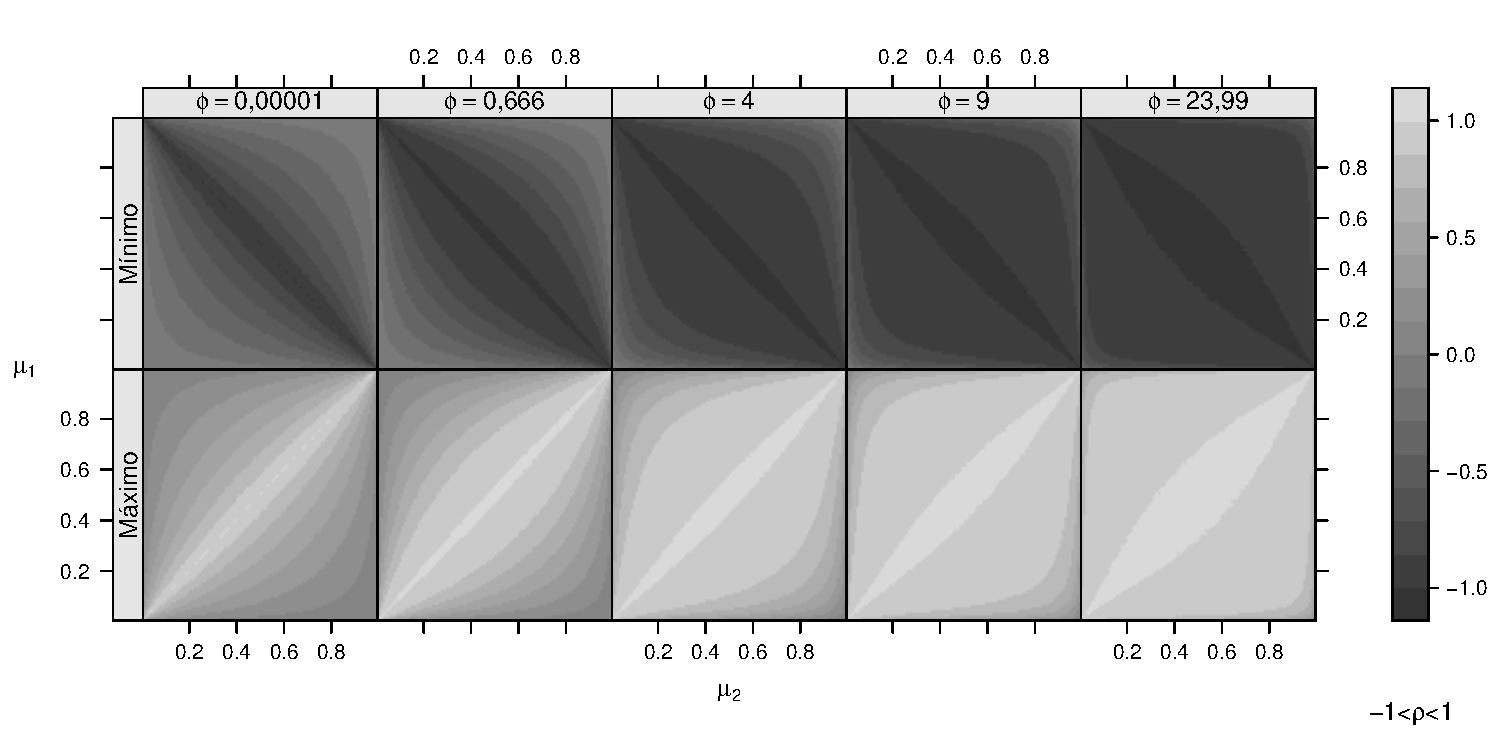
\includegraphics[width=16.0cm,height=7.6cm]{Figure10.pdf}
%   \vspace{-0.7cm}
%   \begin{footnotesize}
%     \centering
%     FONTE: O autor~(2018).
%     \vspace{0.15cm}
%   \end{footnotesize}
%   \label{fig:simulnorta}
% \end{figure}

% \begin{equation}
%   \label{eq:linearPredIQA}
%   g(\mu_{jki}) = \beta_0  + \beta_{1j}~\texttt{local}_{ji} + \beta_{2k}~\texttt{trimestre}_{ki},
% \end{equation}
% \noindent
% Na sequência, ajustou-se o modelo de regressão quase-beta multivariado
% aos dados do IQA, considerando as quatro estruturas acima mencionadas
% além de especificar a função de ligação \textit{logit} para o preditor
% linear~(\autoref{eq:linearPredIQA}).

% END ==================================================================